\section*{Application}
\addcontentsline{toc}{section}{Application}

This repository contains the web publication application of the corpus of manuscript 
sales catalogues. This branch contains the current stable version of the website. See
\texttt{versionX.X.X} for the older versions.

\par\noindent\rule{\linewidth}{0.4pt}
\section*{Getting started :}
\addcontentsline{toc}{subsection}{Getting started :}

\begin{itemize}
\item First, download this repository. Using command lines, clone the repository with : 
\end{itemize}

\begin{listing}[h!]
   \begin{minted}{bash}
git clone https://github.com/katabase/Application.git
cd Application

   \end{minted}
\end{listing}

\begin{itemize}
\item Then, create a virtual environment and activate it : 
\end{itemize}

\begin{listing}[h!]
   \begin{minted}{bash}
python3 -m venv my_env
source my_env/bin/activate

   \end{minted}
\end{listing}

\begin{itemize}
\item Now, you have to install dependencies : 
\end{itemize}

\begin{listing}[h!]
   \begin{minted}{bash}
pip install -r requirements.txt

   \end{minted}
\end{listing}

\begin{itemize}
\item You can finally launch the application : 
\end{itemize}

\begin{listing}[h!]
   \begin{minted}{bash}
python3 run.py

   \end{minted}
\end{listing}

\par\noindent\rule{\linewidth}{0.4pt}
\section*{Use the \texttt{KatAPI}}
\addcontentsline{toc}{subsection}{Use the \texttt{KatAPI}}

\texttt{KatAPI} is an API that allows the automated retrieval of data from the project in 
\texttt{json} or \texttt{xml-tei}. The API allows to revtrieve catalogue entries by author, sale date
and original date of the manuscript; it also allows to retrieve a complete catalogue, or
statistics on one or several catalogues. Finally, it creates custom error messages in \texttt{json}
of \texttt{tei} if an error occurs. For a more complete description, please see the Katabase website.
\subsection*{Quick start}
\addcontentsline{toc}{subsubsection}{Quick start}

The endpoint for the API is \textbf{\texttt{https://katabase.huma-num.fr/katapi?}}. The arguments 
provided by the client are added after this endpoint; the application will process
thoses arguments and send back a response in the requested format (\texttt{json} or \texttt{xml-tei},
the default being \texttt{json}). If there is an error on the client side (unauthorized 
parameters or values) or on the server side (unexpected error), a response will be
issued in \texttt{json} or \texttt{xml-tei} (depending on the client's request) describing the 
query parameters, the time of the query and the error that occured.
\subsection*{Possible query parameters and authorized values}
\addcontentsline{toc}{subsubsection}{Possible query parameters and authorized values}

\noindent{}\textbf{HTTP methods}

The only \textbf{authorized HTTP method} is \texttt{GET}.

\noindent{}\textbf{Possible parameters}

The \textbf{possible parameters} are:

\begin{itemize}
\item \textbf{\texttt{format}}: the format of the API's response body. Possible values are:
\begin{itemize} 
 \item \texttt{json}: \textbf{this is the default value}.
\item \texttt{tei}: return an \texttt{xml-tei} response.
\end{itemize}
\item \textbf{\texttt{level}}: the requested data's level. Possible values are:
\begin{itemize} 
 \item \texttt{item}: data is retrieved at item level. \textbf{This is the default value.}
\item \texttt{cat\_data}: statistical data on one or several catalogues will be retrieved
\begin{itemize} 
 \item this value is incompatible with the \texttt{orig\_date} parameter.
\end{itemize}
\item \texttt{cat\_full}: a complete catalogue encoded in \texttt{xml-tei} will be retrieved
\begin{itemize} 
 \item if this value is provided, then the only other authorized parameters are 		 \texttt{format=tei} and \texttt{id} (with \texttt{id} matching \texttt{CAT-\textbackslash{}d+}).
\end{itemize}
\end{itemize}
\item \textbf{\texttt{id}}: the identifier of the item or catalogue(s) to retrieve (depending on the value of \texttt{level}). If this parameter is provided, data will only be retrieved for a single catalogue or catalogue entry. This parameter cannot be used together with the \texttt{name} parameter. Possible values are:
\begin{itemize} 
 \item if the query is at item level, a catalogue entry's \texttt{@xml:id}. This identifier 	 is a string that matches the pattern: \texttt{CAT\_\textbackslash{}d+\_e\textbackslash{}d+\_d\textbackslash{}d+}.
\item the query is run at catalogue level (\texttt{level=cat\_full} or \texttt{level=cat\_data}), a 	 catalogue's \texttt{@xml:id}. This identifier is a string that matches the pattern: 	 \texttt{CAT\_\textbackslash{}d+}.
\end{itemize}
\item \textbf{\texttt{name}}: if the \texttt{id} parameter is not supplied, the name of the catalogue(s) or catalogue entry(ies) to retrieve. Note that this parameter can, and will, return several items. Possible values:
\begin{itemize} 
 \item if \texttt{level=item}, the \texttt{tei:name} being queried. Only the last name in 	 the \texttt{tei:name} is indexed in the search engine and only this one will yield a 	 result. If a first name and a last name are provided, no result can be yield, since the first name is not indexed.
\item if \texttt{level=cat\_stat}, the catalogue type (to be found in 	 \texttt{(TEI//sourceDesc/bibl/@ana} in the \texttt{xml} representation of a catalogue). 	 Possible values are:
\begin{itemize} 
 \item ``LAC": Vente Jacques Charavay,
\item ``RDA": Revue des Autographes,
\item ``LAV": Catalogue Laveredet,
\item ``AUC": Auction sale
\item ``OTH": not yet in use in our dataset
\end{itemize}
\end{itemize}
\item \textbf{\texttt{sell\_date}}: the sale date for a manuscript or a catalogue. Values must match the regular expression \texttt{\textbackslash{}d\{4\}(-\textbackslash{}d\{4\})?}: a year in \texttt{YYYY} format or a year range in \texttt{YYYY-YYYY} foramat.
\item \textbf{\texttt{orig\_date}}: the date a manuscript item was created. This parameter is only authorized if \texttt{level=item}. Values must match the regular expression \texttt{\textbackslash{}d\{4\}(-\textbackslash{}d\{4\})?}: a year in \texttt{YYYY} format or a year range in \texttt{YYYY-YYYY} foramat. 
\end{itemize}

\pagebreak
\par\noindent\rule{\linewidth}{0.4pt}
\section*{Workflow}
\addcontentsline{toc}{subsection}{Workflow}
\begin{figure}[h]
	\centering
	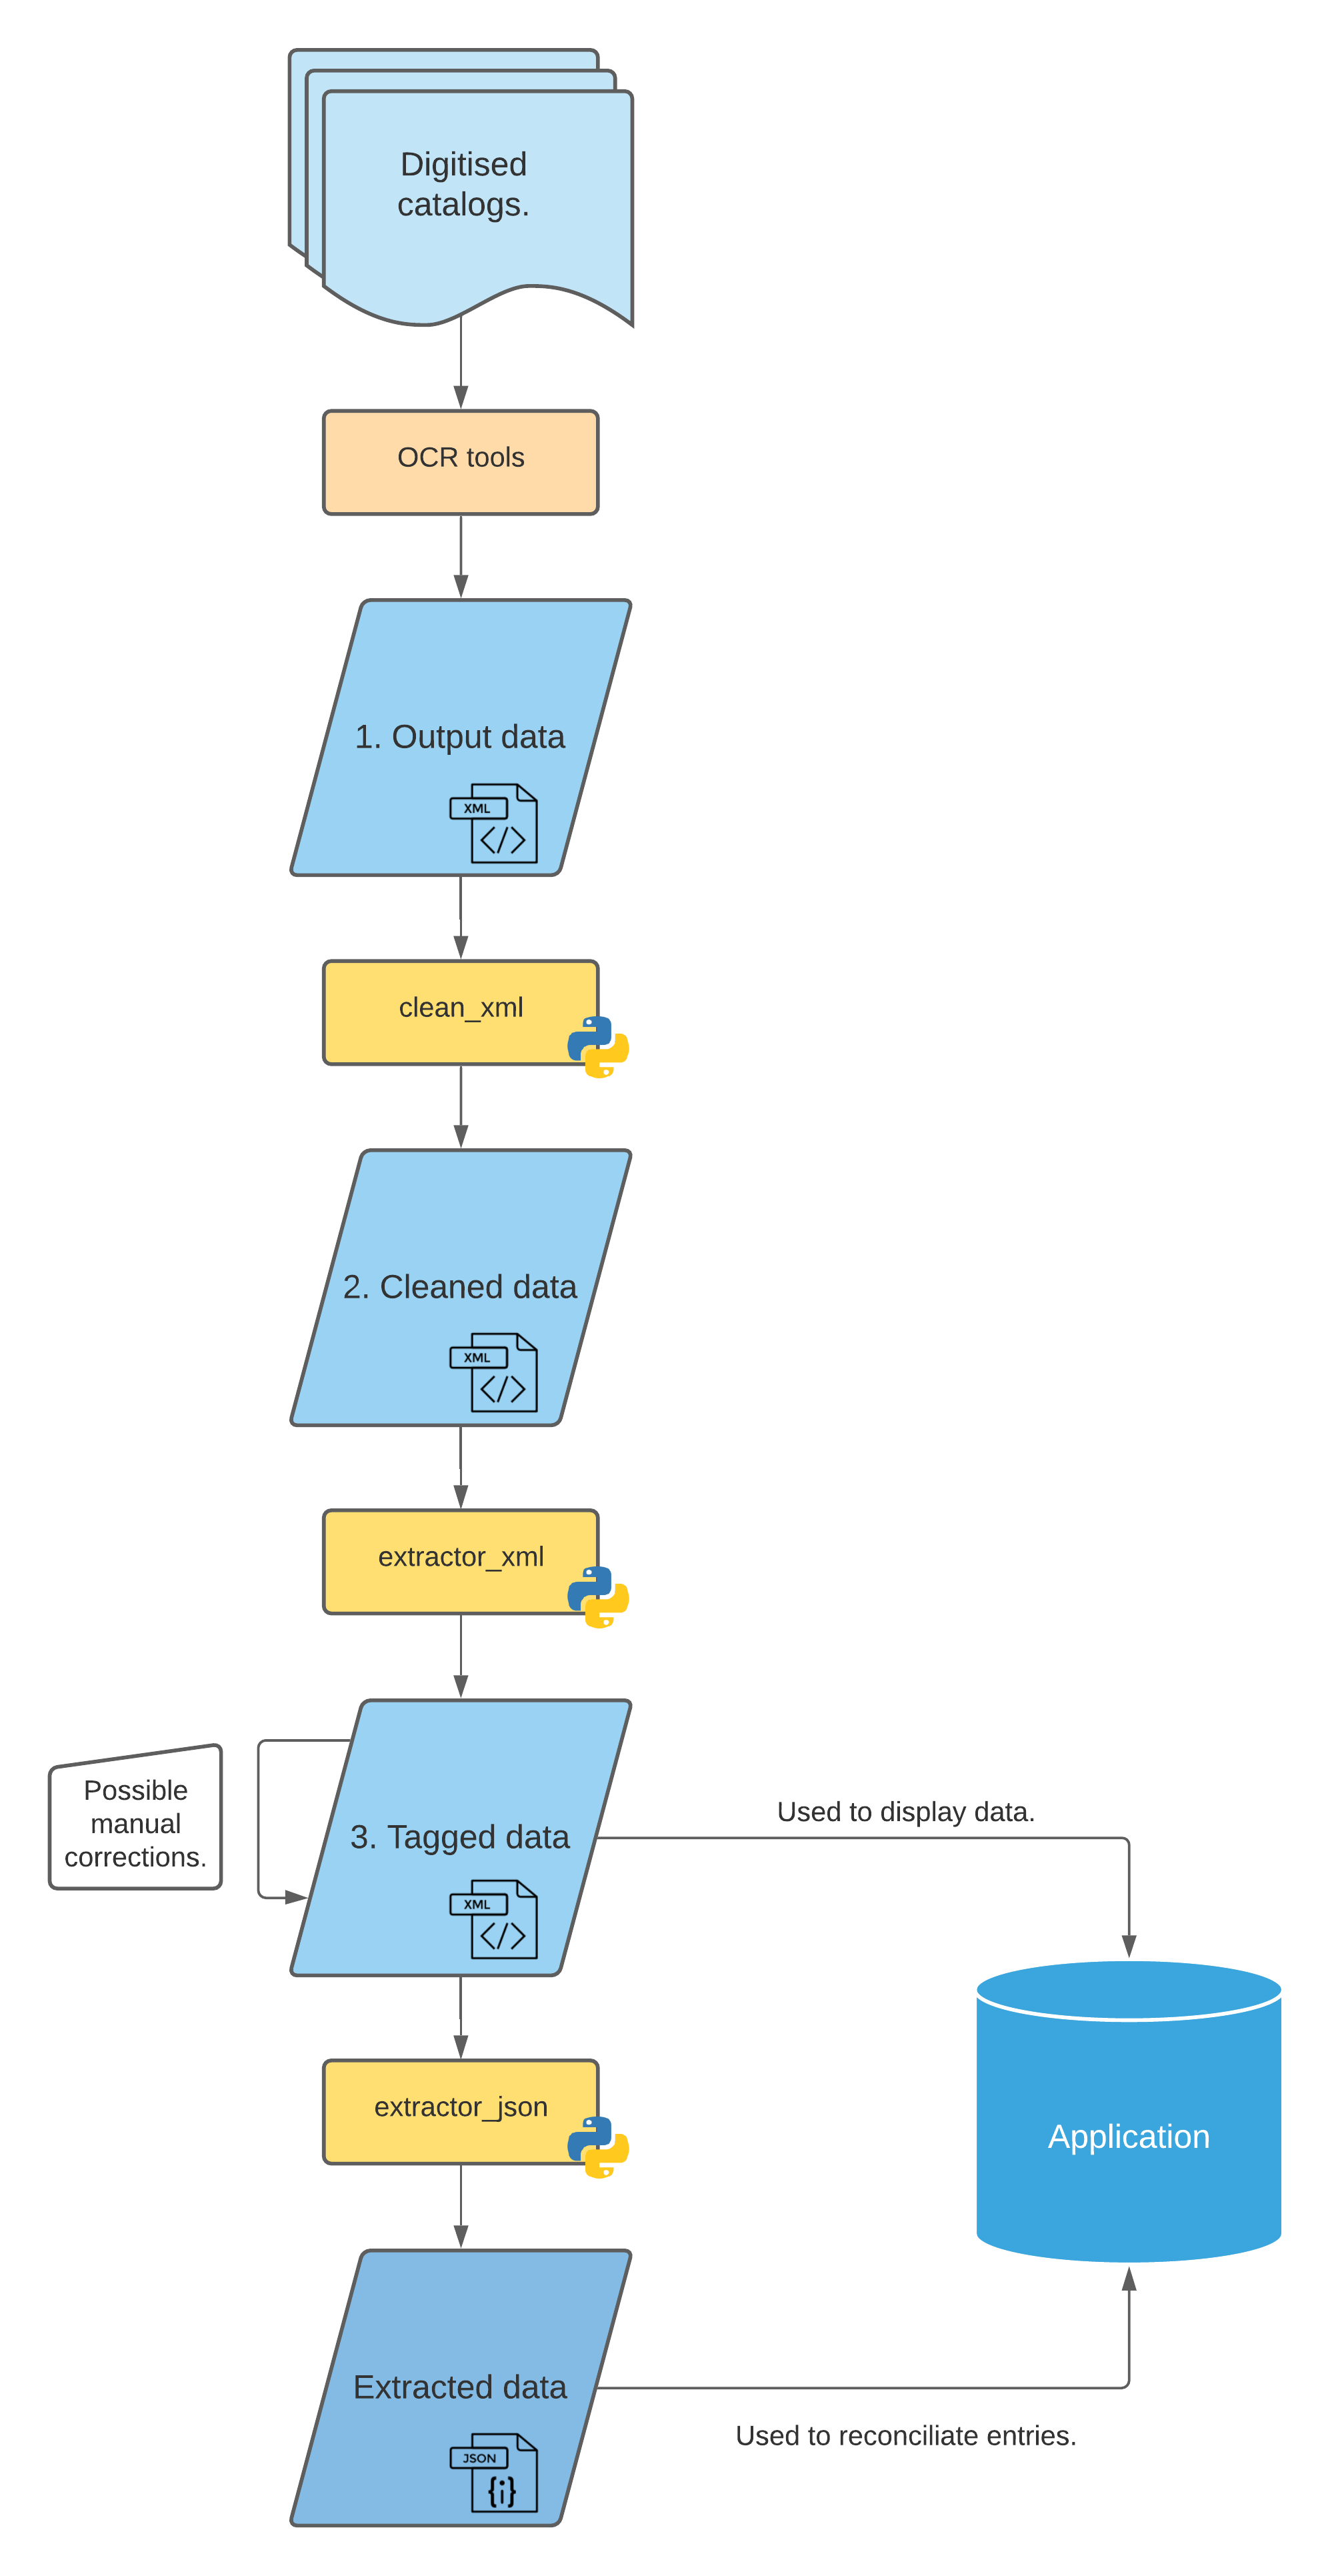
\includegraphics[height=\textwidth]{./annexes/workflow.png}
\end{figure}

\par\noindent\rule{\linewidth}{0.4pt}
\section*{Website updates and description of the git branches}
\addcontentsline{toc}{subsection}{Website updates and description of the git branches}

The structure of the git repository is as follows:

\begin{itemize}
\item \href{https://github.com/katabase/Application}{\texttt{main}} for the current, stable version of the Katabase app
\item \href{https://github.com/katabase/Application/tree/dev}{\texttt{dev}} for the unstable version of the app, in developpment and not running online.
\item \href{https://github.com/katabase/Application/tree/version1.0.0}{\texttt{versionX.X.X}} are archive repositories to document the former versions of the Katabase app. There should be as many of these branches as there are new versions of the website, and their \texttt{X.X.X} code should follow the release numbers. 
\end{itemize}

New additions to the website should be done on \texttt{dev} and tested before being moved to \texttt{main}.
The version of the website visible on \texttt{main} should be the same as the version of the website
online (unless, for reasons out of our control, we can't publish a new version of the website
online, but a new version is ready and won't be changed again). Before merging a new version
of the website from \texttt{dev} to \texttt{main}, the \texttt{main} branch should be moved the \texttt{versionX.X.X}.
A new release should then be created for the updated version of the website.

\par\noindent\rule{\linewidth}{0.4pt}
\section*{Credits}
\addcontentsline{toc}{subsection}{Credits}

The application was designed by Alexandre Bartz and Paul Kervegan with the help of Simon Gabay, Matthias Gille Levenson and Ljudmila Petkovic.

\par\noindent\rule{\linewidth}{0.4pt}
\section*{Cite this repository}
\addcontentsline{toc}{subsection}{Cite this repository}

\section*{Licence}
\addcontentsline{toc}{subsection}{Licence}

The catalogues are licensed under a \href{http://creativecommons.org/licenses/by/4.0/}{Creative Commons Attribution 4.0 International Licence} and the code is licensed under a GNU GPL-3.0 license.
